%\documentclass[trans,handout]{beamer}
\documentclass[trans]{beamer}

%\usepackage{pgfpages}
%\pgfpagesuselayout{4 on 1}[a4paper,landscape,border shrink=5mm]
%\pgfpagesuselayout{2 on 1}[a4paper,border shrink=5mm]

\usepackage[utf8]{inputenc}
\usepackage{graphicx}
\usepackage{multicol}
\usepackage{xcolor}
\usepackage{listings}
\lstset{frame=tb,
  aboveskip=3mm,
  belowskip=3mm,
  showstringspaces=false,
  columns=flexible,
  basicstyle={\small\ttfamily},
  numbers=none,
  numberstyle=\tiny\color{gray},
  keywordstyle=\color{blue},
  commentstyle=\color{green!55!blue},
  stringstyle=\color{purple},
  breaklines=true,
  breakatwhitespace=true,
  tabsize=4
}
\usepackage{hyperref}
\hypersetup{
  colorlinks=true,
  linkcolor=black,
  urlcolor=blue
}
\graphicspath{{figures/}}

\title{
  
\includegraphics[height=.2\textheight]{../abstract/biopython.jpg}\\[1em]
  Biopython Project Update 2017}
\subtitle{}
\author[Sourav Singh]{
  \textbf{Sourav Singh}*, Tiago Ant\~{a}o, Peter Cock, Eric Talevich,\\
  Michiel de Hoon, Wibowo Arindrarto, Leighton Pritchard,\\
  Anuj Sharma, Eric Rasche, Aaron Rosenfeld, Connor T.\\
  Skennerton, Marco Galardini, Markus Piotrowski,\\
  and the Biopython Contributors}
\institute[University of Pune]{* Twitter \& GitHub: @cbrueffer\\Translational Oncogenomics Unit\\Department of Clinical Sciences \\
  Lund University\\
  Sweden\\[1em]
  Bioinformatics Open Source Conference 2017, Prague, CZ \\[1em]
}
\date{May 26th, 2017}


\setcounter{tocdepth}{2}
\setbeamertemplate{caption}{\insertcaption}


% ToC at the beginning of every section
%\AtBeginSection[]
%{
 % \begin{frame} % with <beamer> => doesn't appear in handout mode
  %  \frametitle{Outline} %% Put the title you want, or none!
  %  \tableofcontents[currentsection,currentsection]
 % \end{frame}
%}

\begin{document}

\section{The Biopython Project}
\frame
{
  \frametitle{What is Biopython?}

  \begin{itemize}
  \item Collection of modules for biological computation in Python
  \begin{itemize}
  \item Sequence handling and motifs, parsers, database queries, protein structures, phylogenetics, tool wrappers and lots more
  \end{itemize}
  \item Started in 1999, first release in 2000
  \item Open source and freely available (Biopython license)
  \end{itemize}

  \begin{center}
  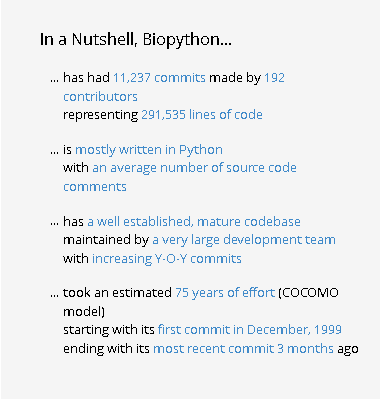
\includegraphics[width=1\textwidth]{openhub-bp-nutshell.png}
  \end{center}
  \small{Source: \url{https://www.openhub.net/p/biopython}}
}
\frame
{
  \frametitle{Stats for the previous 12 months}

  \begin{center}
  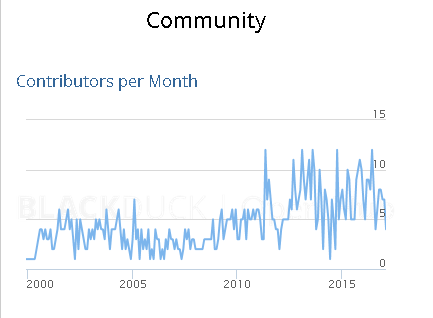
\includegraphics[width=1.0\textwidth]{openhub-bp-community-activity.png}
  \end{center}
  \small{Source: \url{https://www.openhub.net/p/biopython}}
}
\frame
{
  \frametitle{Lots of new contributors!}
  
  \scriptsize{
  \begin{multicols}{3}
  \begin{itemize}
  
  %1.69
  \item Adam Kurkiewicz 
  \item Adam Novak
  \item Adrian Altenhoff
  \item Allis Tauri
  \item Andrew Guy
  \item Andrew Sczesnak
  \item Blaise Li
  \item Brandon Carter
  \item Foen Peng
  \item Francesco Gastaldello
  \item Francisco Pina-Martins
  \item Hector Martinez
  \item Jack Twilley
  \item Jeroen Van Goey
  \item Joshua Meyers
  \item Kurt Graff
  \item Leonhard Heizinger
  \item Marcin Magnus
  \item Maximilian Greil
  \item Michał J. Gajda
  \item Milind Luthra
  \item Oscar G. Garcia
  \item Richard Neher
  \item Sourav Singh
  \item Spencer Bliven
  \item Steve Marshall
  \item Veronika Berman
  
  % after
  \item Aaron Kitzmiller
  \item Bertrand Caron
  \item François Coste
  \item Frederic Sapet
  \item Jimmy O'Donnell
  \item John Kern
  \item Mateusz Korycinski
  \item morrme
  \item Noam Kremen
  \item Rasmus Fonseca
  \item Rodrigo Dorantes-Gilardi
  \item Sacha Laurent
  \end{itemize}
  \end{multicols}
  }
}

%%%%%%%%%%%%%%%%%%%%%%%%%%%%%%%%%%%%%%%%%%%%%%%%%%%%%%%%%%%%%%%%%%%%%%%%%%%%%%%%

\section{New Releases and Beyond}
\subsection*{Release 1.69}
\frame
{
  \center{\LARGE Biopython 1.69 (released 2015-10-21)}
}

\frame
{
  \frametitle{Start of re-licensing plan}
  
  \begin{itemize}
  \item 1.69 marks the start of start of our re-licensing plan, to transition away
from our liberal but unique \emph{Biopython License Agreement} to the widely used \emph{3-Clause BSD License}.
\item The code base-authorship is being reviewed file-by-file, in order to gradually dual license the entire
project.
  \end{itemize}
  
}

\frame
{
  \frametitle{New parser for ExPASy cell line database}
  
  \begin{itemize}
  \item \texttt{Bio.ExPASy}:  
  \begin{itemize}
  \item Cellosaurus cell line database, cell ontologies and cell line catalogues.
  \item Now accessible through the \texttt{Bio.ExPASy} module.
  \end{itemize}
  \end{itemize}
  
  \lstinputlisting[language=Python]{code/expasy.py}
}

\frame
{
  \frametitle{\texttt{Bio.AlignIO} Updates}
  
  \begin{itemize}
  \item \texttt{Bio.AlignIO}: Classes that deal with multiple sequence alignment files.
  \item Support for UCSC MAF format.
  \begin{itemize}
  \item MAF files are now supported using the \texttt{Bio.AlignIO.MafIO} module
  \item Also offers indexed access for large files using SQLite3.
  \end{itemize}
  \end{itemize}
}

\frame
{
  \frametitle{Miscellaneous}

  \begin{itemize}
  \item Miscellaneous bug fixes
  \item Test suite enhancements
  \item Better PEP8 and PEP257 coding style adherence
  \end{itemize}
}

\frame
{
  \frametitle{Biopython 1.69 Contributors}

  \scriptsize{
  \begin{multicols}{2}
  \begin{itemize}
  \item Aaron Rosenfeld
  \item Adam Kurkiewicz (*)
  \item Adam Novak (*)
  \item Adrian Altenhoff (*)
  \item Allis Tauri (*)
  \item Andrew Dalke
  \item Andrew Guy (*)
  \item Andrew Sczesnak (*)
  \item Ben Fulton
  \item Bernhard Thiel (*)
  \item Bertrand Néron
  \item Blaise Li (*)
  \item Brandon Carter (*)
  \item Brandon Invergo
  \item Carlos Pena
  \item Carlos Ríos
  \item Chris Warth
  \item Emmanuel Noutahi
  \item Foen Peng (*)
  \item Francesco Gastaldello (*)
  \item Francisco Pina-Martins (*)
  \item Hector Martinez (*)
  \item Jacek Śmietański
  \item Jack Twilley (*)
  \item Jeroen Van Goey (*)
  \item Joshua Meyers (*)
  \item Kurt Graff (*)
  \item Lenna Peterson
  \item Leonhard Heizinger (*)
  \item Marcin Magnus (*)
  \item Markus Piotrowski
  \item Maximilian Greil (*)
  \item Michał J. Gajda (*)
  \item Michiel de Hoon
  \item Milind Luthra (*)
  \item Oscar G. Garcia (*)
  \item Owen Solberg
  \item Peter Cock
  \item Richard Neher (*)
  \item Sebastian Bassi
  \item Sourav Singh (*)
  \item Spencer Bliven (*)
  \item Stefans Mezulis
  \item Steve Bond
  \item Steve Marshall (*)
  \item Uri Laserson
  \item Veronika Berman (*)
  \item Vincent Davis
  \item Wibowo 'Bow' Arindrarto

  \end{itemize}
  \end{multicols}
  }
}


\frame
{
  \frametitle{Miscellaneous}

  \begin{itemize}
  \item Python 3.3 support deprecated!
  \item Corrections to the \texttt{Bio.Entrez} module (Aaron Rosenfeld)
  \item Corrections to the MMCIF structure parser (João Rodrigues)
  \item Miscellaneous bug fixes
  \item Test suite enhancements
  \item Better PEP8 coding style adherence
  \end{itemize}
}


\subsection*{Current Developments}
\frame
{
  \center{\LARGE What's cooking for Biopython 1.70?}
}


\frame
{
  \frametitle{Biopython 1.70-dev}

  \begin{itemize}
  \item Module \texttt{Bio.AlignIO}
  \begin{itemize}
  \item Support for XMFA file format.
  \item using Bio.AlignIO.MauveIO
  \end{itemize}
  \end{itemize}

}


\frame
{
  \frametitle{Supported Python Versions}
  
  \begin{itemize}
  \item Python 2.7
  \item Python 3.3
  \item Python 3.4
  \item Python 3.5
  \item PyPy 5.0
  \item PyPy3 2.4
  \item Jython 2.7
  \end{itemize}  
}

\section{General Updates}
\frame
{
  \frametitle{Continuous Integration}

  \begin{itemize}
  \item TravisCI
  \item Experimentation with Build Stages for CI testing.
  \begin{itemize}
  \item Codecov.io (test coverage)
  \item Quantified Code (metrics and automatic pull requests)
  \item Landscape.io (``health score'')
  \end{itemize}
  \item Currently enabled by default: Codecov.io, Quantified Code
  \end{itemize}

  \begin{columns}
  \column{0.4\textwidth}
  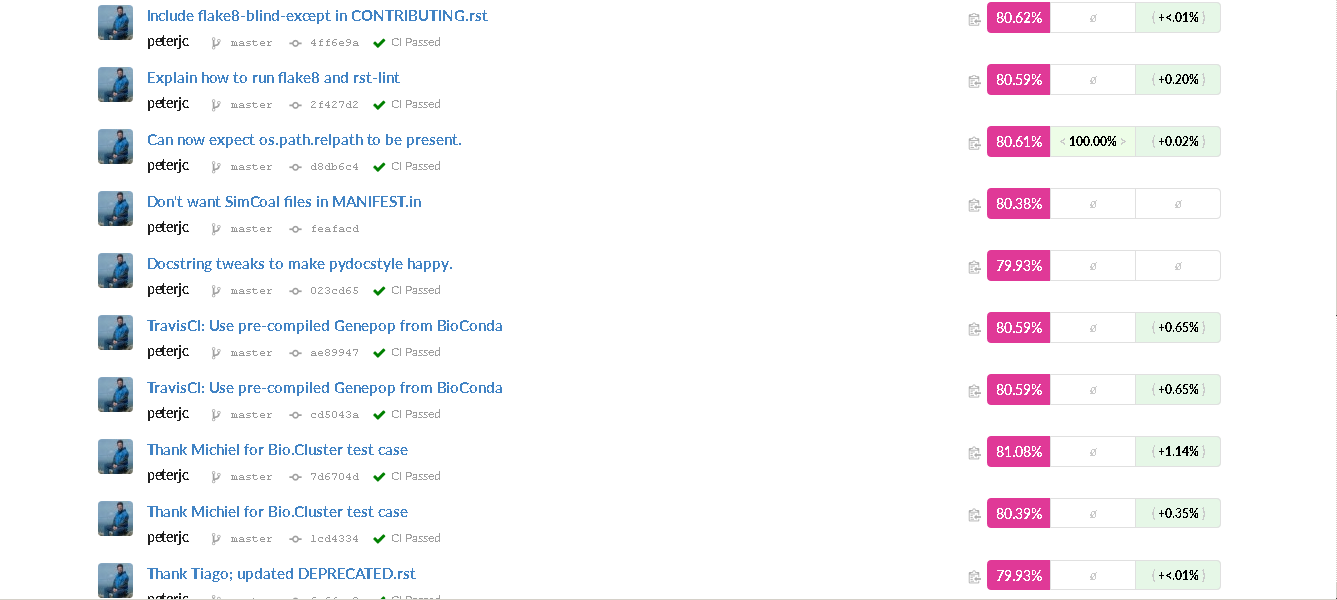
\includegraphics[width=1\textwidth]{bp-codecov.png}
  \column{0.6\textwidth}
  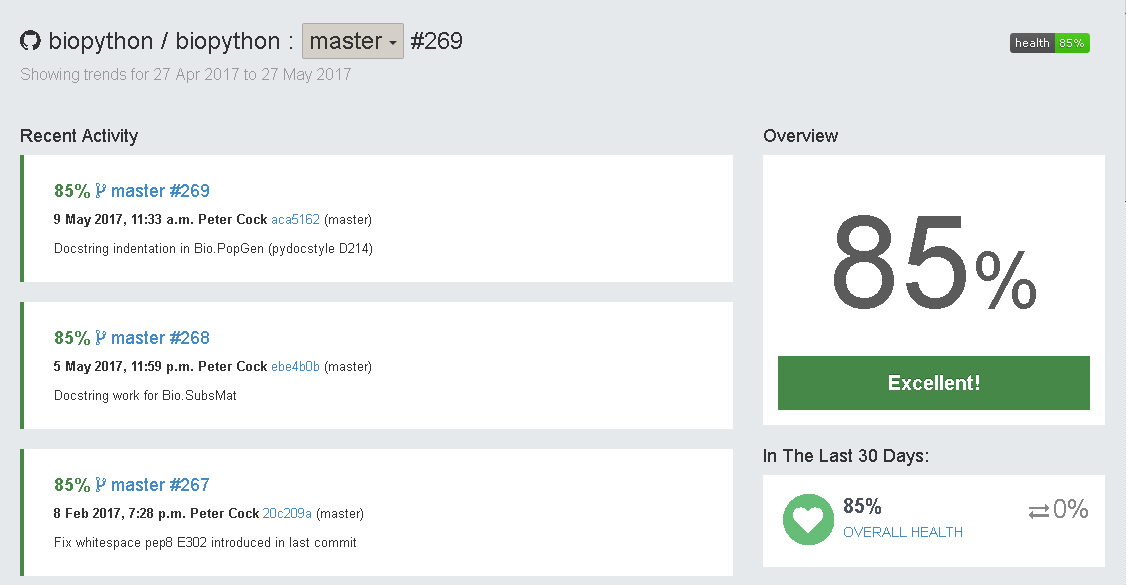
\includegraphics[width=1\textwidth]{bp-landscape.png}
  \end{columns}
}

\section{Conclusion}
\frame
{
  \frametitle{Conclusion}

  \begin{itemize}
  \item Lots of new contributors
  \item Lots of new stuff
  \item Turn new contributors into recurring ones
  \item Biopython 1.70 in the near future
  \end{itemize}
}

\frame
{
  \frametitle{Acknowledgements}

  \begin{minipage}{1\textwidth}
  \begin{columns}
  \column{0.5\textwidth}
  \begin{itemize}
  \item Peter Cock
  \item Biopython Community
  \end{itemize}
  \column{0.5\textwidth}
  
\includegraphics[width=0.8\textwidth]{biopython.jpg}
  \end{columns}
  \end{minipage}

  \vspace{0.5cm}

  \begin{minipage}{1\textwidth}
  \begin{columns}
  \column{0.2\textwidth}
  
\includegraphics[width=0.5\textwidth]{github-logo.jpg}
  \column{0.2\textwidth}
  
\includegraphics[width=0.5\textwidth]{travisci-logo.png}
  \column{0.2\textwidth}
  
\includegraphics[width=0.5\textwidth]{codecov-logo.png}
  \column{0.2\textwidth}
  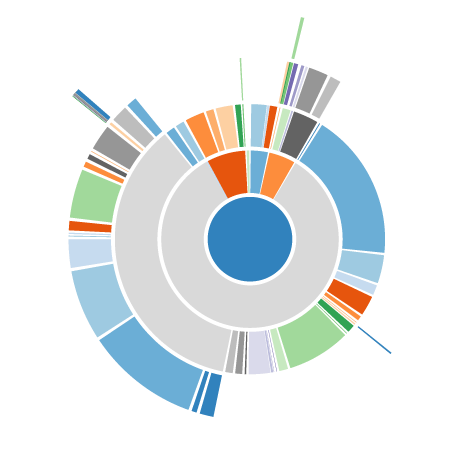
\includegraphics[width=0.5\textwidth]{quantifiedcode-logo.png}
  \column{0.2\textwidth}
  
\includegraphics[width=0.5\textwidth]{obf-logo.png}
  \end{columns}
  \end{minipage}
}

\section*{Acknowledgements}
\frame
{
  \frametitle{Resources!}

  %\begin{center}
  Website:\\
  \begin{itemize}
  \item \url{http://biopython.org}
  \end{itemize}

  Repositories:\\
  \begin{itemize}
  \item Main: \url{http://github.com/biopython/biopython}
  \item Website: \url{https://github.com/biopython/biopython.github.io}
  \end{itemize}

  Mailing lists:
  \begin{itemize}
  \item General list: \url{biopython@biopython.org}
  \item Developers list: \url{biopython-dev@biopython.org}
  \end{itemize}

  Biostars:
  \begin{itemize}
  \item \url{https://www.biostars.org/t/biopython/} (``biopython'' category)
  \end{itemize}
  %\end{center}
}

\end{document}
